%
% File coling2014.tex
%
% Contact: jwagner@computing.dcu.ie
%%
%% Based on the style files for ACL-2014, which were, in turn,
%% Based on the style files for ACL-2013, which were, in turn,
%% Based on the style files for ACL-2012, which were, in turn,
%% based on the style files for ACL-2011, which were, in turn, 
%% based on the style files for ACL-2010, which were, in turn, 
%% based on the style files for ACL-IJCNLP-2009, which were, in turn,
%% based on the style files for EACL-2009 and IJCNLP-2008...

%% Based on the style files for EACL 2006 by 
%%e.agirre@ehu.es or Sergi.Balari@uab.es
%% and that of ACL 08 by Joakim Nivre and Noah Smith

\documentclass[11pt]{article}
\usepackage{coling2014}
\usepackage{times}
\usepackage{url}
\usepackage{latexsym}
\usepackage{todonotes}
\usepackage{graphicx}
%\usepackage[style=authoryear]{biblatex}

\definecolor{dark-cornflower-blue-2}{RGB}{17,85,204}
\definecolor{dark-green-2}{RGB}{56,118,29}
\definecolor{dark-blue}{RGB}{0,0,100}

\newcommand{\sk}[1]{{\color{dark-green-2} #1}}
\newcommand{\dr}[1]{{\color{dark-cornflower-blue-2} #1}}
\newenvironment{sketch}{\color{dark-green-2}}{\ignorespacesafterend}
\newenvironment{draft}{\color{dark-cornflower-blue-2}}{\ignorespacesafterend}

%\setlength\titlebox{5cm}

% You can expand the titlebox if you need extra space
% to show all the authors. Please do not make the titlebox
% smaller than 5cm (the original size); we will check this
% in the camera-ready version and ask you to change it back.


\title{AI Essay}
% suggestions:
%	Intelligence and simulation of minds
%	Conscious machines


\author{First Author \\
  Affiliation / Address line 1 \\
  Affiliation / Address line 2 \\
  Affiliation / Address line 3 \\
  {\tt email@chalmers} \\\And
  Second Author \\
  Affiliation / Address line 1 \\
  Affiliation / Address line 2 \\
  Affiliation / Address line 3 \\
  {\tt email@chalmers} \\\And
  Third Author \\
  Affiliation / Address line 1 \\
  Affiliation / Address line 2 \\
  Affiliation / Address line 3 \\
  {\tt email@chalmers} \\}

\date{}

\begin{document}

\todo{Come up with another title for the essay}

\maketitle
\begin{abstract}
\sk{
In this essay, we discuss the question of whether machines can have minds. We start off by introducing some of the arguments and ideas that have been proposed on the subject during the last 70 years, from Turing to Nagel and Searle. We then try to define what a mind is, showing some examples from the animal kingdom. In the discussion ..., e.g. the Turing test and the Chinese room \todo{Bjorn, finish this}
}
\todo{possible keywords: mind, ...}
\end{abstract}

\section{Introduction}
\label{sec:introduction}

It all started with the question "Can machines think?". We as human civilisation have been creating tools to solve problems since the beginning of our time. As we grew better at creating tools and collecting them together, we were able to build more and more complex machines upon each other. Then came the computer, a machine first designed as a computational tool, which we later gave the ability to improve itself. Inevitably, we started to feel the uncertainty of what this can lead to.

Alan Turing avoided answering this question by introducing an imitation game experiment \cite{turing1950computing}. Can machines behave indistinguishably as human from another human observer's perspective? This experiment itself raised another discussion among computer scientists and philosophers. As researchers in various areas improved from the time of Turing, instead of asking if machines think, we would like to explore the question of whether machines can have minds.


% How to use colors %%%
%\sk{This is sketchy text, ie Green.}
%
%\dr{This is draft text, ie Blue}
%
%\begin{sketch}
%You can also write Green sketch like this...
%\end{sketch}
%
%\begin{draft}
%...and draft text like this.
%\end{draft}

%%%%%%%%%%%%%%

\subsection{Strong versus weak AI}

Before we dive into the discussion regarding machines with their minds, a clear framework should be illustrated in order to achieve the most fruitful discussion. We often hear "strong AI" and "weak AI" in the domain of artificial intelligence research, but these phrases can actually have two different meanings. Since the terms overlap, they are sometimes accidentally confused. We would like to clear the distinctions here.

\subsubsection*{Strong and weak AI used in computational theory of mind}

John Searle is often regarded as the first person to use the term "strong AI" in this definition in his "Minds, brains, and programs" \cite{searle1980minds}. According to John Searle, "strong AI" claims that programs (or programmed computers) that correctly maps the right input to the right output, should be regarded as possessing a mind just like humans possess minds. On the other hand, "weak AI" (discussed more in Section \ref{sec:what_is_a_mind}) claims this mapping is merely an imitation of mind and so cannot be accounted as a real mind. Searle's famous Chinese room thought experiment, which is explained in more detail in Section \ref{sec:chinese_room}, serves as a refutation to strong AI claims. In this thought experiment, Searle introduced the concept of "intentionality" which is not possible to model or include in any program. A man in this Chinese room can perform a task perfectly by following the given instructions and rules while not knowing any Chinese. No intentionality at all is involved in the tasks carried out. 
%Another way of understanding the difference is by looking into the actual actions carried out in the Chinese room experiment, one can describe the instruction-following guy only access the syntax rules of Chinese, not the semantics of Chinese he/she been given.

\subsubsection*{Strong and weak AI used to describe the ability to solve general problems within a single agent}

Sometimes also referred to as full AI, strong AI in this branch can be defined as an agent which can demonstrate the ability to perform any intellectual task that humans are capable of \cite{kurzweil2005singularity}. That is, an agent can solve tasks that are not predetermined on a level matching a human. If there exists an artificial intelligence agent which can pass the Turing test, one can classify it as strong AI or full AI because it demonstrates the ability to perform tasks in terms of natural language dialogue equivalent (or indistinguishable from a third person's observation) to human level. 
%Passing the Turing test might not suggest the agent can solve "any" task humans can, which can be too vague to achieve (infinite list of task).
However, the general consensus is that general intelligence must accomplish the following:
\begin{enumerate}
\item reasoning
\item learning
\item planning
\item natural language communication
\item Knowledge representation (KR) 
\end{enumerate}

%We will refer to the first definition of strong AI as Searle's idea on strong AI and the second as Turing's. 
Although discussion in either one of these branch often leads to some common arguments from another branch, it is better to clarify at beginning.

\subsection{What is a mind?}
\label{sec:what_is_a_mind}

\subsubsection*{Does simulated minds count as real mind?}

As we mentioned earlier, Searle refuted the claim that simulation of mind, itself should be counted as a real mind. Till today this argument still remains a topic of debate. So why do people waffle about whether a simulation of mind can be attributed as a real mind or not? Another famous question of philosophy, the mind-body problem, could be linked to this simulation problem. The 17th-century philosopher Ren{\'e} Descartes is commonly acknowledged to be the first person who formalised this problem \cite{descartes1641meditationes}: "How could the immaterial mind (or soul) influence the material body?". Descartes also discussed where the boundary between the material world and the immaterial world is, if one regard information flow as input and mind as processor of information. Like most philosophical problems, the answer to the mind-body problem seems to depend largely on one's personal belief.

%\subsubsection*{Border between mindful creation and not?}
\subsubsection*{Intelligence in animals}

In order to better understand the concept of minds, we take a look at intelligence in some known organisms. 
%We assume that humans have minds since we are capable of conscious thought and abstract reasoning. 
Many animals are known to exhibit intelligent behaviour in both individuals and communities. For example, many species of fish, bird and some mammals are able to periodically travel great distances to the location of their birth once a year. Other species such as dogs, dolphins and ants are well known for their social behaviour.

Mackintosh noted that crows had the ability to carry information from experiment to experiment while pigeons were notoriously bad at this, seemingly starting over from scratch \cite{mackintosh1988animals}. He refuted the then common idea that intelligence in animals could be ordered using the evolutionary tree, i.e. the "phylogenetic hierarchy". 
Crows are also known to craft and use tools to gather food and defend against predators \cite{emery2004crows}. In an experiment, a crow could reason about which tool to use as well as making tools from new materials (metal wire) when no twigs were available.
Furthermore, crows use strategy in both caching their own food for future use and pilfering food caches of other birds. 
Emery and Clayton also compared the brains of crows and chimpanzees.
The ratio of brain size and the rest of the body is about the same and both species have an enlarged brain center for cognitive thought: neocortex in apes and nidopallium in corvids (crows). However the structure of the nidopallium is very different from the neocortex of the apes. We thus draw the conclusion that complex cognition can be brought about by different (brain) architectures resulting in similar levels of intelligence.

\subsubsection*{Which animals have minds?}

Now that we have discussed some intelligent behaviour of various animals, we can try to distinguish which of them have minds and which do not. We can argue that humans have minds since we are capable of conscious thought and abstract reasoning. On the other hand bacteria may not possess minds as far as we can observe since they seem not be able to learn and remember. However, one can argue that bacteria learn as communities by mutation and that individuals reason about which action to take from their chemical perception of their surroundings. So even for a simple organism such as bacteria, to decide if they have minds is not trivial. Here we assume bacteria are mindless since they seem to depend more on random mutations than conscious actions.

It has been noted in the past that ordering animals' intelligence in a single dimension lacks proper foundation \cite{mackintosh1988animals} so we will not make this assumption here. However many dimensions are needed to present the intelligence of animals, there must be some classifying function between humans and bacteria that categorizes which have minds and which do not. The problem is that there seems to be little consensus in how to draw such a distinction.

One can argue that humans are unique in being able to evolve as a species in a much faster rate than evolution. Cultural changes, advances in medicine and technology can all be considered a conscious evolution of the species. While stray dogs may not be able to construct metro stations of their own, they can learn how to use them to navigate their neighbourhoods, not so differently from their fellow human passengers \cite{moskowDogs}. Crows have been recorded to drop nuts on pedestrian crossings and eating the crushed content when the traffic lights switches in favour of the pedestrians \cite{crowNuts}. These innovative and adapting behaviours can be considered proof that dogs and crows have minds.

%Another view of mind is that of meaning. Humans typically perform recreational activities such as creating and enjoying art, music and fiction. For many humans, these activities are regarded as meaningful even if they lack a direct purpose.

A more general view would be that some set of aspects of intelligence such as spatial intelligence, long-term memory, learning abstract concepts, language and social behaviour would be sufficient or necessary for possessing a mind. Exactly which concepts are required and to what extent is a matter of debate.

%\subsubsection*{(Maybe a way to separate): Purpose-driven OR Meaning driven?}
 
% \begin{draft}
%Our discussion regarding to strong/weak AI or Chinese room experiment started with ideas from video clip shown in class "Humans need not apply" \cite{grey2014humans}. Horses, once extensively used worldwide by human, are completely replaced by auto-mobiles. This analogy is used to compare current situation of human labours and near-future artificial intelligence replacing us. Could we become the next horses and eliminated from job market? Judging by technology today, the answer is almost certain \todo{certain in what way?}. But we humans are different from horses fundamentally in terms of roles on earth, this is why we have created civilisations and horses have not. We used horses for the purpose of transportation because they are good at going forward (provided with some incentives and/or punishments). If one sees this process from abstract point of view, the process of getting a horse to walk from Paris to Nantes is very much similar to process of getting our AI agent from Arad to Bucharest \todo{relating to the pathfinding example, or?}. A purpose-driven agent who only exists for serving limited collection of purposes (most commonly single purpose). Although in some occasions in our lives we read Shakespeare just to pass some final exams (very much like the horse previously mentioned \todo{I don't see the connection to horses here. /Björn}), most of the time we dive into deeper, more abstract processes of thinking for no direct causal result. A meaning driven agent who proceed carrying out tasks even no heuristics or feedbacks given. 

%The difference of a meaning driven behaviour is clearly different from purpose driven ones, but its rarely found in nature with exception of human activities (and some specific activities of particular mammals like dolphin). Neocortex can be related to these high level consciousness but having neocortex doesn't implies meaning driven behaviours \todo{What is neocortex?}. 
%\end{draft}

%%%%%%%%%%%%%%%%%%%%%%%%%%%%%%%%%%%%%%%%%%%%%%%%%%%%%%%%%%%%
\section{Discussion}
\label{sec:discussion}

\subsection{How to test if an agent possesses a mind?}

Previously we noted that depending on the definition of mind, several animals could be thought of as having a mind or not. So instead of attempting to resolve this ambiguity we will attempt 
%Since it is quite hard to know what a mind is in general we instead attempt 
to answer the question of whether a machine can possess a human mind, that is to think like a human.

\begin{figure}
\centering
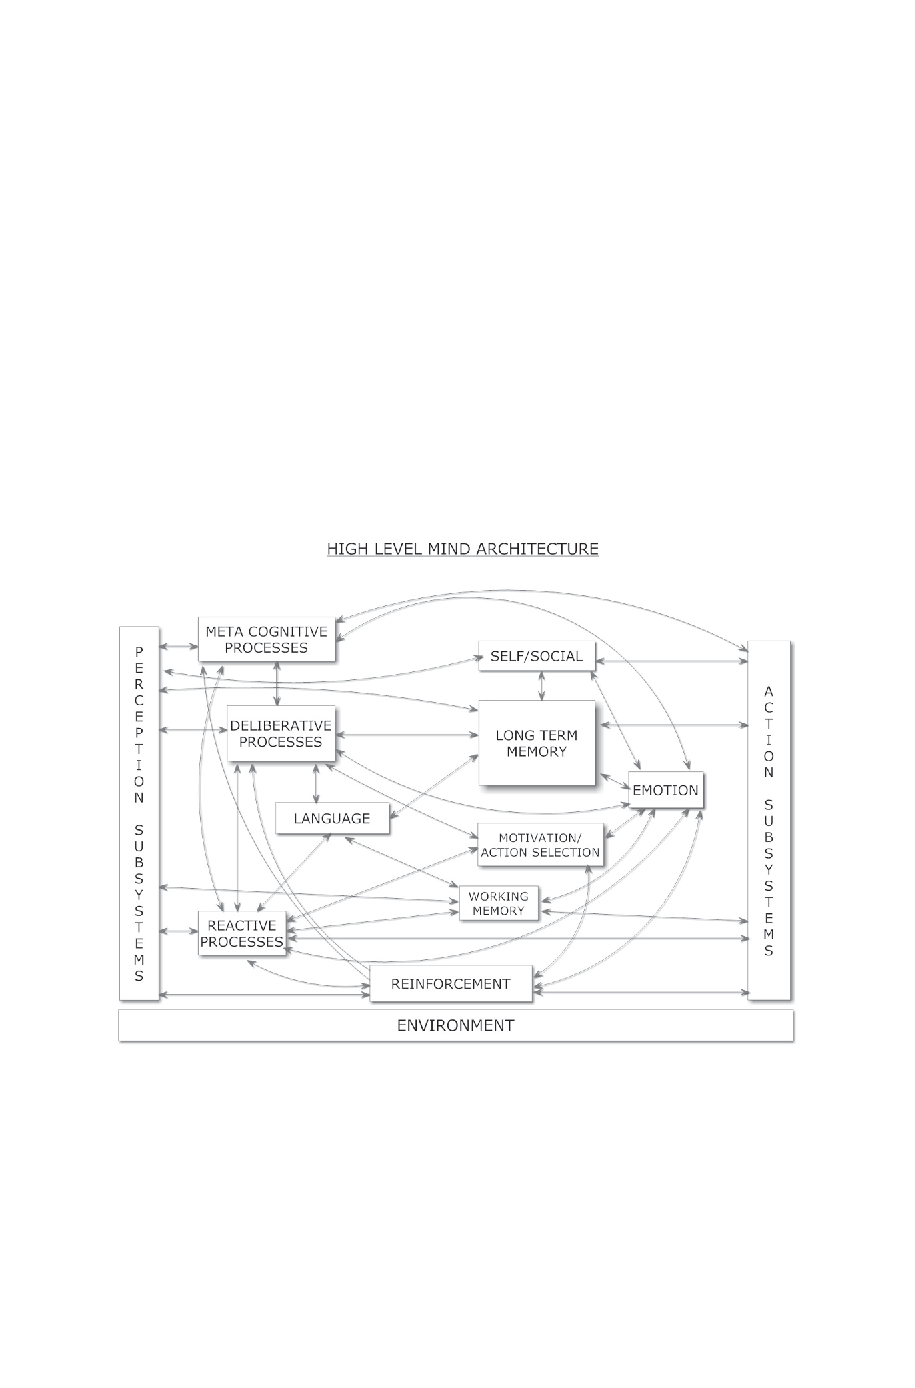
\includegraphics[scale=1.0]{mindStructure.pdf}
\caption{Model architecture of human mind as proposed by Goertzel \cite{goertzel2012agi}.}
\label{fig:mindArchi}
\end{figure}

\subsubsection*{Architecture of the human mind}
Goertzel collected a lot of research from psychology and neurology to form a conceptual model of the human mind from the different theories \cite{goertzel2012agi}. The resulting diagram can be found in figure \ref{fig:mindArchi}. \todo{Jeff, do something here}

%\begin{sketch}

% To determine if machines can possess minds, one can go through some formulated tests:
%\end{sketch}

\subsubsection*{Testing AGI (Artificial General Intelligence)}
Goertzel notes that there are several tests for assessing whether an agent has achieved a human level of AGI \cite{goertzel2012agi}. The most classical one would be the Turing test which statistically tests if the robot could be indistinguishable from a human \cite{turing1950computing}. A human judge would ask several, possibly connected, questions over a text chat to both a robot and a human participant. The judge would then guess which of the two participants really is human.

Another, more difficult, test would be to let a robot enroll in a university \cite{goertzel2012agi}. The robot would succeed if it was able to obtain a degree given the same conditions of passing as the human students.

Goertzel also listed some tests that could be assumed to require human intellect but could also be solved by a "narrow AI", i.e. specific to the task, \cite{goertzel2012agi}. One of these tests: "to be able to play an arbitrary video game based on experience only" was recently achieved by Google on the Atari game platform \cite{googleAtari}.

\dr{Goertzel also mentions that it is very difficult to measure when research is halfway to the goal since all components in the architecture of the mind are so interdependent: even if only one or two parts are missing, the agent would probably not behave even close to a mind \cite{goertzel2012agi}.} \todo{Perhaps move this sentence?}

\subsubsection*{Understanding minds}

The tests above only test the behaviour of an agent, that is AGI. When it comes to minds, consciousness and understanding others, Nagel made an interesting point \cite{nagel1974like}. He argues that a human can never understand what it is like to be a bat: We can try to imagine sleeping upside down, navigating with sonar and "catching insects with our mouths" but that would only result in what it would be like for oneself to be a bat, which is fundamentally different from what it would be like for a bat to be a bat.
% we can only imagine what it would be for us to be a bat which is different from understanding what it is like for a bat to be a bat.

%A related example would be how does one’s native tongue (ex Swedish) sound like to a foreign person (ex Chinese), we can only imagine what it would be like because we only know what it sounds like to a Swedish person. 

If we accept Nagel's argument, one can draw the parallel to computers. Thus a bat expert might be able to predict and even imitate a bat while not being able to understand it internally. Likewise, a computer could possibly imitate and predict human behaviour whilst not understanding humans emotionally. For example, things like laughter, grief and art could possibly be predicted or emulated but not internally understood.

\subsubsection*{Chinese Room Experiment}
\label{sec:chinese_room}

In any case, even if a machine would successfully understand all abstract parts of being human, it could be very hard to tell from just a smart imitating machine. Searle illustrated this in his famous thought experiment: the Chinese room \cite{searle1980minds}. If an agent that speaks English natively but doesn't understand any Chinese is sealed away in a room together with a list of very thorough instructions of how to manipulate some input characters (presumably) written in Chinese, he might be able to produce some Chinese text but it doesn't mean he understands what he is doing. However, the people on the outside might not be able to distinguish that agent from a native Chinese speaker, assuming the instructions are sufficiently detailed and intelligently designed. Likewise, if a computer successfully could understand humans, we couldn't really tell the difference of that from a list of intelligent instructions executed by a thorough but non-understanding agent.

\subsection{How does a simple mind arise?}

What might be considered as \textit{simple minds} can arise in, among others, animals and robotics. Of course, this depends on which definition of 'mind' is used, a question which definitely is not trivial. On one hand, these 'minds' display complex and seemingly intelligent behaviours. But on the other hand it is sometimes also possible to describe and explain these complex behaviours using rather simple explanations, like the food-finding capabilities of \textit{E. Coli} bacteria or the navigation methods used by the desert ant \textit{Cataglyphis Fortis} \cite{wahde2015autonomous}. This falls into what is called \textit{complex systems}: complex behaviours arising from simple components. Examples of this, some of which are described below, are social insects and even single-celled organisms.

\subsubsection*{Slime mould}

Slime mould are unicellular amoeba which, when food is in short supply, can form into networks that coordinate and display behaviours similar to animals with simple brains\todo{Bjorn: find references. John Tyler Bonner?}. This is extraordinary, since the individual cells are not known to have the ability to think. Yet somehow a large collection of these individuals are able to display a degree of intelligence when put together, something which can be seen in the example with slime mould. An experiment in which a mass of slime mould was placed in an artificial environment (representing the area around Tokyo) showed that the slime mould was able to find an efficient way of connecting the major cities in the Greater Tokyo Area \cite{tero2010rules}. The generated map was strikingly similar to the rail network that already is in use in the Tokyo area.
% http://scienceblogs.com/notrocketscience/2010/01/21/slime-mould-attacks-simulates-tokyo-rail-network/

\subsubsection*{Bee drones}

The societies of social insects are known to display complex behaviours, for example when searching for food or new homes. Researchers are now trying to create robots which are inspired by social insects. At the University of Harvard, a research team is developing RoboBees, microrobots with a size and behaviour similar to those of real bees \cite{robobees2015}. The hope is that these robots will be able to work in areas such as artificial pollination, search and rescue operations, weather monitoring and so on. The RoboBees, though rather simple robots on their own, will be able to collaborate as a "colony" in order to efficiently solve tasks. \todo{How do the robots achieve this?}
% http://robobees.seas.harvard.edu

At the universities of Sheffield and Sussex, researchers are cooperating in the Green Brain Project with the aim of building a model that mimics the brain of a bee \cite{greenbrain2015}. The goal is to achieve a better understanding in how honeybee brains work and at the same time find improvements for the methods used in controlling autonomous flying vehicles. So far, the researchers have been able to simulate parts of a bee's brain and upload it to an UAV (quadcopter), allowing it to fly and use simple navigation to avoid running into obstacles.
% http://greenbrain.group.shef.ac.uk/research/

%%%%%%%%%%%%%%%%%%%%%%%%%%%%%%%%%%%%%%%%%%%%%%%%%%%%%%%%%%%%
\section{Conclusion}
\label{sec:conclusion}

\subsection{Does it matter?}

\subsubsection*{Before we start, you have to know they don't care!}
Simulation of intelligence or real intelligence is in many sense not important issue for AI researchers working on delivering programs that finish designated tasks. As much as you wouldn't care if a screwdriver is actually a simulated solution or a real solution as long as it fixes your IKEA beds. AI research is therefore needed as it produces more tools for solving our problems in life, and some of these problems are practically unsolvable without these tools. We now pose a nice question to ponder: a screwdriver is a handy tool but in the wrong hand could be a weapon to harm others. Did the inventor of the screwdriver think of this perspective? Wouldn't it be more safe to not release this potentially dangerous version of screwdriver and instead keep refining it until a more harmless version is invented?
  
Another question worthy considering would be: "If a computer, provided with the correct software, can be considered as a creation with a mind (and in some degree, consciousness), would it be a crime of murder if the plug is pulled out?"

%\begin{sketch}
%\subsubsection*{Assuming a computer with proper software accounts as mindful creation, we wont be able to find out!}
%
%\subsubsection*{Does physical differences impose different level of mutual understanding?}
%\end{sketch}

\begin{sketch}
\subsubsection*{$(\mbox{simple mind})^n = \mbox{complex mind}$?}
Brains are too complex to recreate or mimic at the time of writing, yet if it is possible to show our direction of \todo{Bjorn, look through this} work is on the right track? Examples shown in attempts on recreating simple minds maybe can offer us some confidence. One can either build very simple units (replicating a slime mould or a neuron) or assemble meta-complex brains like bee's. Given previous studies on composition, or to say components, of human mind, it could be possible even with smaller scale of minds, like bee's, can lead us to some association of certain functions of mind to its corresponding circuitry. Or by focusing on single simple cell replications, like slime mould, and grouping large quantities of these simple agents for performing complex behaviour in order to help us understand how to transform basic communication of individual agents into higher level pattern which in turns trigger complex behaviours. Although there exists technological limitation, for instance a maximum computation power per single chip before causing meltdown on chip itself, we can still combine many known principles from development of modern computer systems in attempt to explore more possibilities. 
\end{sketch}

\subsubsection*{Our limits need not apply}
\begin{draft}

if we regard programs  as form of intelligence and mindful thing, machine intelligence shouldn't be confined (or defined) by limitations of humans. Maybe one can argue computers will never be able to understand true semantics of our natural languages, but this could be very narrow view. Our natural languages are result of cultural evolution separated by geographical boundaries, and if we review history of mankind, the flaws in natural language causing misunderstanding or semantic mismatch costed us dearly. Yet all civilisation throughout the world seems to reach one common \todo{wording: common $\rightarrow$ unified?} syntax when it comes to mathematics. The connection from its syntax to semantics are so absolute that we still use zero to represent very same concept when zero was invented. Computers and programs are born in world of math, binary or not, there exists no doubt that computers are much capable than humans in field of numbers. Needless to say the speed of computation carry out by computers, easily reaching to petaflop at the time of writing, can never be achieved by our biological limits. 

It is truth saying human brains are most complex masterpiece of nature, evolution made our brain perfect to handle any happening situation around us. We can see the world and filter out most critical information and process under amazing low power consumption. While machines still have huge difficulty identifying heels from sneakers, one has to consider the fundamental differences between human and machine. Analog information is easy task for us because we've survived in such analog world for thousands of years, but you can't perceive current temperature up to 3 decimal precision. 

Embracing such perspective, and one will find huge potential in development of machines. As mentioned, all our cultures are geologically separated, so are all the individuals of mankind. Our communication forms are still very limited, even with aid from machines. Given the power of almost instantaneous connection, evolution curve of machine must exceed ours. 
\end{draft}

%\todo{Leif, add something to conclusion}
\subsection{Final words}
\begin{draft}

As we have seen, it can be hard to define what a mind really is and how to test it. As Goertzel noted, detecting partial progress is even harder. On the bright side, this may mean that we are closing of achieving a conscious machine than we think but it can also discourage people from trying. From the top side, we can look at components of the human mind and discuss how to emulate them; from the bottom side, we can simulate simple brains. When the two approaches go deep enough to meet, a working mind may not be far even if it is not at a human level.

However, if a successful simulation of mind really is a mind in itself and therefore is subject to ethics, is a philosophical question. Furthermore, if a robot mind is created it will not necessarily be human or close to human but considering human history, that may turn out to not be such a bad thing.

\end{draft}



%%%%%%%%%%%%%%%%%%%%%%%%%%%%%%%%%%%%%%%%%%%%%%%%%%%%%%%%%%%%
% include your own bib file like this:
\bibliographystyle{acl}
\bibliography{references}

\end{document}
